\documentclass[10pt, a4paper, twocolumn]{article}

% --- 页面排版设置 ---
\usepackage[a4paper, left=1.5cm, right=1.5cm, top=2.54cm, bottom=2.54cm, columnsep=0.4cm]{geometry}
\usepackage{mathptmx} % 官方指定 Times 字体
\usepackage{titlesec} % 控制标题格式
\usepackage{caption}  % 控制图表标题
\usepackage{graphicx} % 插入图片
\usepackage{booktabs} % 三线表
\usepackage{amsmath}  % 数学公式
\usepackage{amssymb}  % 数学符号 (mathbb)
\usepackage{fancyhdr} % 页脚设置
\usepackage{tabularx} % 自适应列宽表格
\usepackage{array}    % 表格列格式
\usepackage{enumitem} % 列表间距控制
\usepackage{setspace} % 行距微调
\usepackage{afterpage} % 强制浮动体页面控制
\usepackage{multirow}
\usepackage{float}    % 提供 [H] 强制图表就地放置

% --- 标题层级格式重定义 ---
\titleformat{\section}{\fontsize{12pt}{14pt}\bfseries}{\thesection}{1em}{}
\titleformat{\subsection}{\fontsize{10pt}{12pt}\itshape}{\thesubsection}{1em}{}
\titleformat{\subsubsection}[runin]{\fontsize{10pt}{12pt}\itshape}{\thesubsubsection}{1em}{}[ :]
\titlespacing*{\section}{0pt}{8pt}{4pt}
\titlespacing*{\subsection}{0pt}{6pt}{3pt}
\titlespacing*{\subsubsection}{0pt}{4pt}{2pt}

\captionsetup[figure]{font=small, position=bottom, justification=centering, skip=4pt}
\captionsetup[table]{font=small, position=top, justification=centering, labelsep=space, skip=4pt}

% 减小公式上下间距
\setlength{\abovedisplayskip}{6pt}
\setlength{\belowdisplayskip}{6pt}
\setlength{\abovedisplayshortskip}{3pt}
\setlength{\belowdisplayshortskip}{3pt}

% 减小浮动体间距
\setlength{\textfloatsep}{8pt plus 2pt minus 2pt}
\setlength{\floatsep}{6pt plus 2pt minus 2pt}
\setlength{\intextsep}{6pt plus 2pt minus 2pt}

% 仅保留页脚的页码
\pagestyle{plain}

% 图片路径
\graphicspath{{./}}

\begin{document}

% --- 顶部通栏区域 ---
\twocolumn[{

    \begin{center}
      {\fontsize{18pt}{20pt}\selectfont\textbf{JITTER MULTI-COMPONENT DECOMPOSITION VIA SPARSE BAYESIAN LEARNING}\par}

      \vspace{1.5em}

      {\fontsize{10pt}{12pt}\selectfont\textit{\textbf{Qihang Sun$^{1}$, Secondname A. Author$^{2}$, Corresponding C. Author$^{3*}$}}\par}

      \vspace{1em}

      {\fontsize{10pt}{12pt}\selectfont\textit{$^{1}$Department of Electronic Engineering, First University, City, Country\\
      $^{2}$Department of Computer Science, Second Institute, City, Country\\
      $^{3}$Department of Research, Third Institute, City, Country\\
      $^{*}$email address of corresponding author}\par}
    \end{center}

    \vspace{1.5em}

    \noindent\textbf{Keywords:} JITTER DECOMPOSITION; PERIODIC JITTER; SPARSE BAYESIAN LEARNING; REDUNDANT DICTIONARY; SIGNAL INTEGRITY\par

    \vspace{1.5em}

    \noindent{\fontsize{12pt}{14pt}\selectfont\textbf{Abstract}}\par
    \vspace{0.4em}

    \noindent Accurate decomposition of jitter components from time interval error (TIE) sequences is a critical step in signal integrity assessment of high-speed digital communications. Existing frequency-domain decomposition methods locate the periodic jitter (PJ) frequency via FFT peak detection and then fit the amplitude using least squares. However, the non-uniform edge spacing of PRBS signals causes the TIE sequence to violate the uniform sampling assumption of FFT, producing a systematic frequency estimation bias that misaligns the PJ amplitude estimate and propagates errors into the other components.

    To address this limitation, this paper proposes a jitter decomposition method based on Sparse Bayesian Learning (SBL): a redundant dictionary with independently configurable frequency resolution is constructed, and the Automatic Relevance Determination (ARD) mechanism selects active dictionary columns in place of FFT peak detection. To accelerate the inference, Fast Relevance Vector Machine (FastRVM) is first applied on a coarse grid to localise the active frequencies, and ARD then performs fine-grained inference within the resulting neighbourhoods.

    Experimental results show that, compared with the above baseline method, the proposed approach consistently constrains the PJ estimation error within 0.5~ps across the wide frequency range of 100~kHz--15~MHz, and effectively suppresses error propagation from frequency bias into the ISI and RJ components, thereby validating the effectiveness and robustness of the proposed method.


    \vspace{2.5em}
}]

% ==========================================
% --- 正文双栏开始 ---
% ==========================================

\section{Introduction}

As the data transmission rate of high-speed digital communications continues to increase, systems impose increasingly stringent constraints on timing accuracy and signal integrity. Jitter, as the core factor affecting bit error rate (BER), has become a key metric in signal integrity assessment~\cite{balestrieri_review_2019}. Capturing time interval error (TIE) sequences with an oscilloscope and accurately decomposing each component is the foundation for evaluating system performance and locating interference sources~\cite{chen_methodology_2023}. Based on physical origins and statistical characteristics, total jitter (TJ) is conventionally decomposed into random jitter (RJ) and deterministic jitter (DJ), the latter being further classified into inter-symbol interference (ISI), duty cycle distortion (DCD), and periodic jitter (PJ)~\cite{tripathi_review_2018}.

Existing jitter decomposition methods can be broadly classified into three categories: statistical-domain, time-domain, and frequency-domain. Statistical-domain methods, represented by tail fitting~\cite{deng_jitter_2024} and the Dual-Dirac model~\cite{fang_jitter_2024,peng_jitter_2025}, enable rapid separation of RJ and DJ but lack explicit modelling of the pattern dependence of ISI. Time-domain methods such as time lag correlation (TLC)~\cite{dou_jitter_2006} separate correlated and uncorrelated jitter components via correlation functions but cannot directly extract PJ frequency information. Frequency-domain methods, such as FFT-based spectral peak detection~\cite{yamaguchi_fft_2007}, intuitively reveal the spectral structure of PJ but likewise lack explicit modelling of ISI pattern dependence. Recent deep learning-based approaches~\cite{ren_jitter_2021} have also made progress, but typically rely on large amounts of labelled data and offer limited interpretability.

Duan et al.~\cite{duan_fast_2019} proposed a least-squares decomposition method based on a linear superposition model of TIE, which locates the PJ frequency via FFT peak detection and then fits the amplitude using least squares (hereinafter referred to as LS-FFT). This method incorporates PJ, ISI, DCD, and RJ into a unified linear model and can simultaneously estimate all component amplitudes from a small number of TIE samples. However, its accuracy presupposes accurate FFT frequency estimation. TIE is defined only at data transition edges, while consecutive identical bits in real data patterns produce no transitions, so adjacent TIE samples are not equally spaced on the time axis and violate the uniform sampling assumption of FFT, causing the FFT peak to deviate from the true PJ frequency (as illustrated in Fig.~\ref{fig:nonuniform_sampling}). Furthermore, when the PJ frequency falls between two DFT grid points, the picket-fence effect further aggravates this bias. Fitting the PJ component with the shifted frequency misaligns the basis with the true signal, causing amplitude misestimation that propagates errors into the ISI and RJ components.

\begin{figure}[htbp]
    \centering
    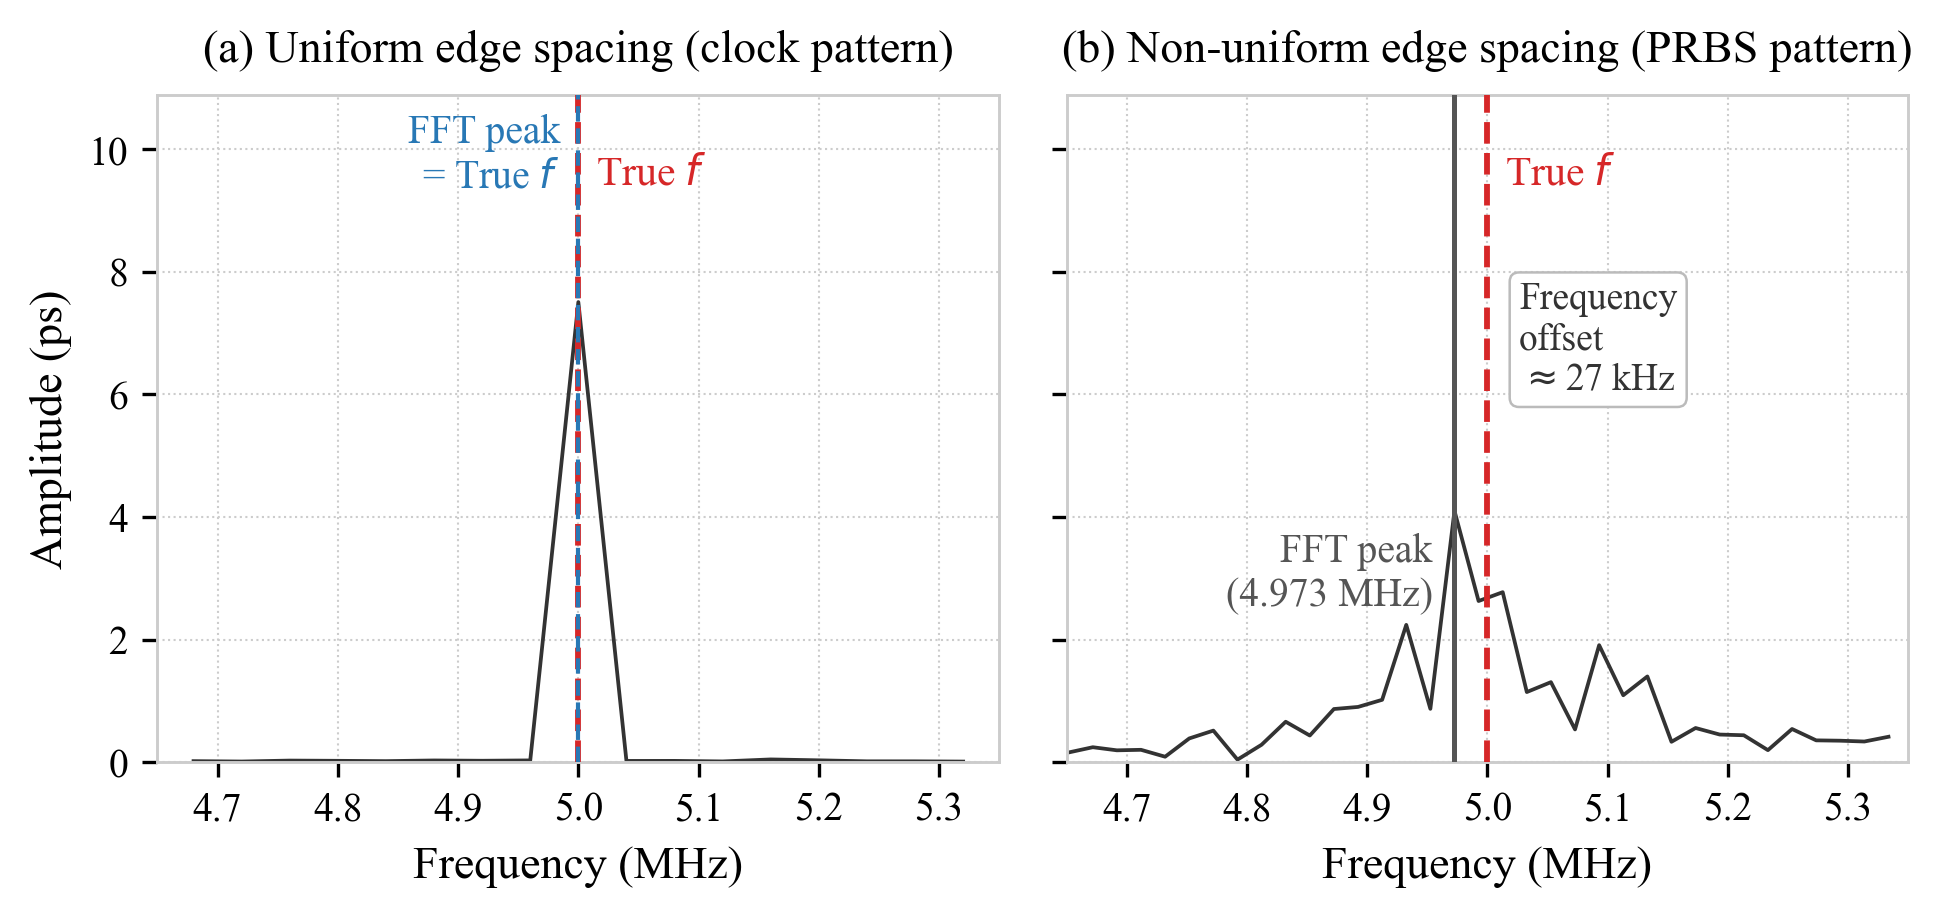
\includegraphics[width=0.88\linewidth]{fig1_nonuniform_sampling.png}
    \caption{Non-uniform edge distribution of a PRBS signal.}
    \label{fig:nonuniform_sampling}
\end{figure}

To address these problems, this paper proposes a jitter multi-component decomposition method based on Sparse Bayesian Learning (SBL). Building on the linear superposition model of Duan et al.~\cite{duan_fast_2019}, the proposed method constructs a redundant dictionary using the true transition instants and replaces the single-frequency column with a large set of candidate frequencies whose spacing and count are no longer constrained by the number of sampling points. The Automatic Relevance Determination (ARD) mechanism of SBL directly selects the true PJ frequencies from the redundant dictionary, without requiring FFT peak detection, thereby avoiding the frequency estimation bias caused by non-uniform sampling and the picket-fence effect.


\section{Signal Model and Dictionary Construction}

\subsection{Linear TIE model}

The TIE at the $k$-th transition edge can be decomposed, according to its physical origin, into a linear superposition of deterministic components and random noise:

\begin{equation}
y(k) = y_{PJ}(k) + y_{ISI}(k) + y_{DCD}(k) + v(k) \tag{1}
\end{equation}

where $v(k)$ comprises random jitter and observation noise. Stacking the TIE samples over $N$ transition edges in matrix form~\cite{duan_fast_2019}:

\begin{equation}
\mathbf{y} = [\mathbf{A}(f_0) \mid \mathbf{B} \mid \mathbf{C}]\,\mathbf{x} + \mathbf{v} \tag{2}
\end{equation}

The PJ sub-matrix $\mathbf{A}(f_0) \in \mathbb{R}^{N \times 2}$ has columns $d_n \cos(2\pi f_0 n/f_s)$ and $d_n \sin(2\pi f_0 n/f_s)$, where $d_n$ is the transition indicator (1 at a transition, 0 otherwise); the DCD sub-matrix $\mathbf{B} \in \mathbb{R}^{N \times 1}$ is set to $+1$ for rising edges and $-1$ for falling edges; the ISI sub-matrix $\mathbf{C} \in \mathbb{R}^{N \times 2^L}$ buckets the rows by the history pattern within memory depth $L$, placing a $1$ in the column corresponding to the current pattern of each row.

The accuracy of the solution to (2) hinges on whether $\mathbf{A}(f_0)$ reflects the true phase structure of the PJ component on the TIE sequence. The phase term $2\pi f_0 n/f_s$ in the $n$-th row of $\mathbf{A}(f_0)$ approximates the $n$-th transition as a uniformly sampled point at $n/f_s$. Under PRBS patterns, however, consecutive identical bits produce no transition, so adjacent transitions are not equally spaced in time; the phase bias introduced by this approximation causes the FFT-based estimate of $f_0$ to deviate systematically from its true value, and the bias is propagated through the least-squares fit to the PJ and the other component amplitudes.

\subsection{Redundant frequency dictionary}

Rather than relying on FFT peak detection, this paper places $K$ candidate frequencies within the target band, constructs the dictionary column for each candidate using the actual transition arrival times $t_n$, and identifies the active frequencies by SBL. Here $t_n$ is the ideal arrival time of the $n$-th transition edge: under PRBS testing the transmitted pattern is known, so the transition positions can be determined directly from the pattern as $t_n = \mathrm{edge\_index}(n)/f_s$; this information is already available when extracting the TIE sequence. A cosine--sine basis-column pair is then constructed for each candidate frequency $f_i$:

\begin{equation}
\begin{aligned}
\mathbf{h}_{c,i} &= [d_1\cos(2\pi f_i t_1), \ldots, d_N\cos(2\pi f_i t_N)]^T \\
\mathbf{h}_{s,i} &= [d_1\sin(2\pi f_i t_1), \ldots, d_N\sin(2\pi f_i t_N)]^T
\end{aligned} \tag{3}
\end{equation}

A PJ component with arbitrary initial phase can be represented linearly as $a_i \mathbf{h}_{c,i} + b_i \mathbf{h}_{s,i}$, converting nonlinear phase estimation into a linear coefficient problem. Concatenating the basis-column pairs of the $K$ candidate frequencies horizontally yields the PJ sub-dictionary:

\begin{equation}
\mathbf{H}_{PJ} = [\mathbf{h}_{c,1}, \mathbf{h}_{s,1}, \ldots, \mathbf{h}_{c,K}, \mathbf{h}_{s,K}] \in \mathbb{R}^{N \times 2K} \tag{4}
\end{equation}

The spacing and count of candidate frequencies $f_1, \ldots, f_K$ are not constrained by the DFT grid $\Delta f = f_s/N$ and may be chosen flexibly according to the target band. Concatenating $\mathbf{H}_{PJ}$ with $\mathbf{B}$ and $\mathbf{C}$ yields the global redundant dictionary:

\begin{equation}
\mathbf{H} = [\mathbf{H}_{PJ} \mid \mathbf{B} \mid \mathbf{C}] \in \mathbb{R}^{N \times M}, \quad M = 2K + 1 + 2^L \tag{5}
\end{equation}

After solving for the coefficient vector $\hat{\mathbf{x}}$, the physical quantity of each component is extracted as follows. The coefficient pair $(\hat{a}_i, \hat{b}_i)$ at an active frequency $f_i$ gives the peak-to-peak PJ amplitude:

\begin{equation}
\mathrm{Pk\text{-}Pk}_{PJ} = 2\sqrt{\hat{a}_i^2 + \hat{b}_i^2} \tag{6}
\end{equation}

The DCD and ISI peak-to-peak values are $\mathrm{Pk\text{-}Pk}_{DCD} = 2|\hat{x}_{DCD}|$ and $\mathrm{Pk\text{-}Pk}_{ISI} = \max(\hat{\mathbf{x}}_{ISI}) - \min(\hat{\mathbf{x}}_{ISI})$ respectively; the RMS RJ is estimated from the fitting residual:

\begin{equation}
\hat{\sigma}_{RJ} = \sqrt{\frac{\|\mathbf{y} - \mathbf{H}\hat{\mathbf{x}}\|_2^2}{N - P}} \tag{7}
\end{equation}

where $P$ is the number of active columns in $\mathbf{H}$.

Adjacent candidate-frequency columns of $\mathbf{H}$ are highly correlated, $\mathbf{H}^T\mathbf{H}$ is severely ill-conditioned, and a direct least-squares solution is numerically unstable. In practice, the number of simultaneously active PJ interference sources is limited, so only a few entries of the coefficient vector are non-zero; the problem reduces to identifying these non-zero columns from the candidate set and estimating their values. Sparse Bayesian Learning (SBL) provides a probabilistic inference framework for such sparse recovery problems~\cite{tipping_sparse_2001}.


\section{SBL-Based Jitter Decomposition Algorithm}

Although the frequency resolution of the redundant dictionary is not constrained by the number of samples, finer resolution implies more candidate columns. Constructing a fine dictionary with thousands of columns directly would force ARD to update all columns jointly, with computational cost growing quadratically with the column count, rendering a single inference prohibitively slow. FastRVM, by contrast, updates one column at a time and is computationally efficient on large coarse-grid dictionaries, but the coarse spacing limits its frequency resolution. This paper therefore performs inference in two steps: FastRVM is first used to localise the rough intervals containing the PJ frequencies on a coarse grid, and a fine dictionary is then constructed within those intervals so that ARD can yield accurate frequency and amplitude estimates. Both steps identify active frequency columns by maximising the marginal likelihood, and the complete algorithm pipeline is shown in Fig.~\ref{fig:flowchart}.

\begin{figure}[htbp]
    \centering
    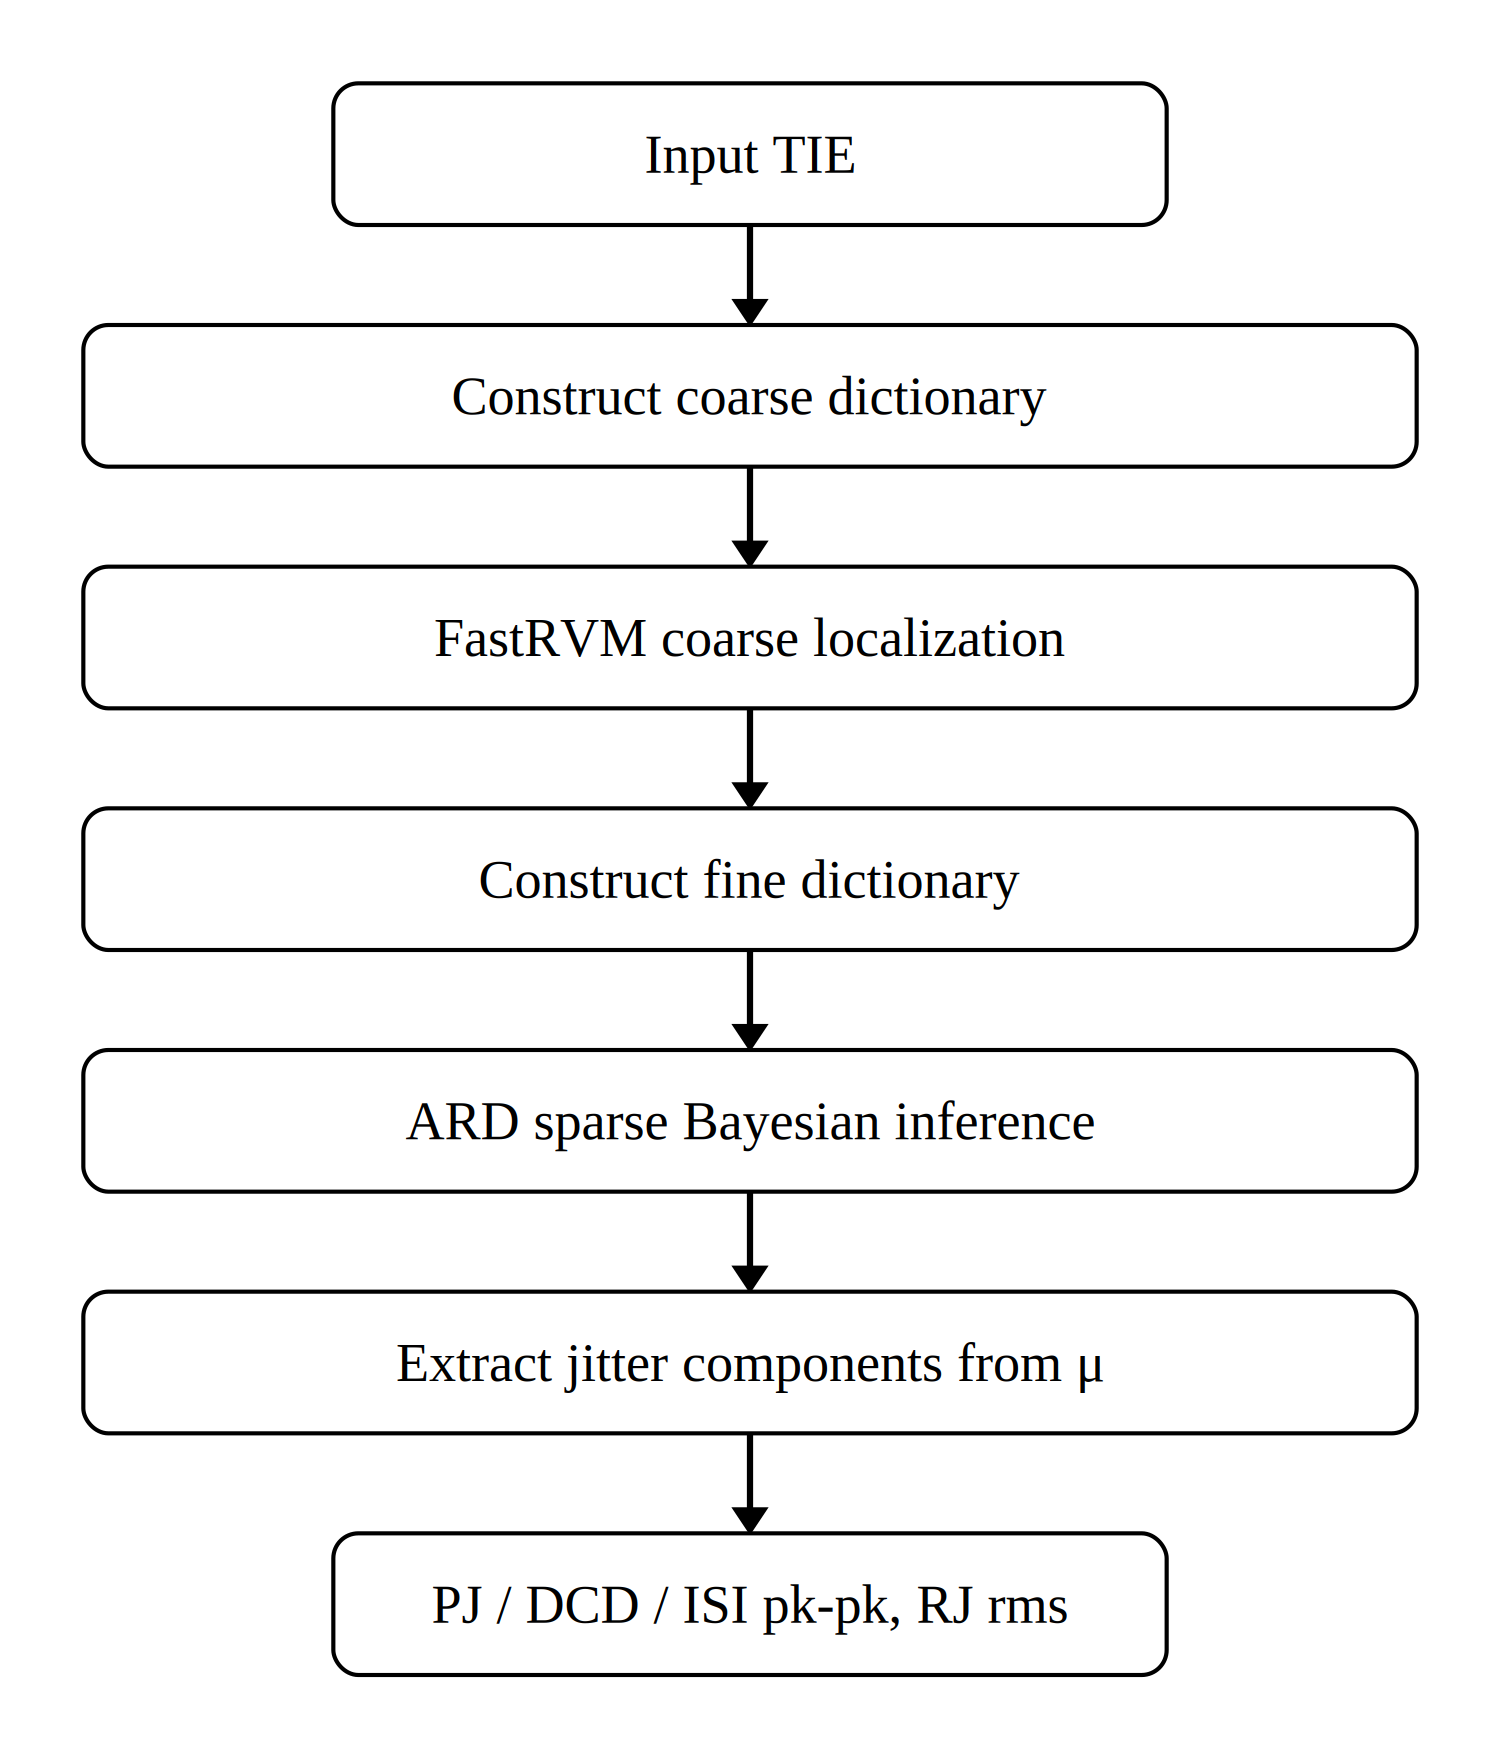
\includegraphics[width=0.82\linewidth]{fig3_flowchart.png}
    \caption{Flowchart of the SBL-based jitter decomposition algorithm.}
    \label{fig:flowchart}
\end{figure}

\subsection{FastRVM coarse localisation}

The purpose of coarse localisation is to determine the rough intervals containing the PJ frequencies over the full band 100~kHz--15~MHz.

SBL assigns an independent zero-mean Gaussian prior to each component of the coefficient vector $\mathbf{w}$~\cite{tipping_sparse_2001}:

\begin{equation}
w_i \sim N(0, \alpha_i^{-1}) \tag{8}
\end{equation}

where $\alpha_i$ is a precision hyperparameter; $\alpha_i \to \infty$ effectively removes the corresponding column. The set $\{\alpha_i\}$ is estimated from the data by maximising the marginal likelihood, and after convergence only a few columns retain finite $\alpha_i$, achieving sparse recovery.

One hundred candidate frequencies are uniformly placed over 100~kHz--15~MHz; a 200-column PJ sub-dictionary is constructed according to (3)--(4) and concatenated with $\mathbf{B}$ and $\mathbf{C}$ to form a 233-column coarse global dictionary. FastRVM sequential sparse inference~\cite{faul_analysis_2001} is applied to this dictionary. The observation model is $\mathbf{y} = \mathbf{H}\mathbf{w} + \boldsymbol{\varepsilon}$ with $\boldsymbol{\varepsilon} \sim N(\mathbf{0}, \sigma^2 \mathbf{I})$.

FastRVM does not iterate over all columns simultaneously but maintains an active column set $A$, initially empty, and at each step decides whether to include or exclude a single column. When examining the $i$-th column, the quality factor $Q_i$ and sparsity factor $S_i$ with respect to the current residual are computed:

\begin{equation}
Q_i = \mathbf{h}_i^T \boldsymbol{\Phi}^{-1} \mathbf{y}, \quad S_i = \mathbf{h}_i^T \boldsymbol{\Phi}^{-1} \mathbf{h}_i \tag{9}
\end{equation}

where $\mathbf{h}_i$ is the $i$-th dictionary column and $\boldsymbol{\Phi} = \sigma^2\mathbf{I} + \mathbf{H}_A\boldsymbol{\Lambda}_A^{-1}\mathbf{H}_A^T$ is the marginal covariance matrix corresponding to the current active set $A$. $Q_i$ reflects the contribution of the $i$-th column to fitting the residual; $S_i$ reflects the energy of that column itself. The Sparsity--Quality criterion is then constructed~\cite{faul_analysis_2001}:

\begin{equation}
\theta_i = Q_i^2 - S_i \tag{10}
\end{equation}

$\theta_i > 0$ indicates that the fitting improvement from this column exceeds the complexity cost of including it; the column is added to the active set and $\alpha_i$ is updated by the closed-form maximiser of the marginal likelihood:

\begin{equation}
\alpha_i^{\mathrm{new}} = \frac{S_i^2}{\theta_i} \tag{11}
\end{equation}

$\theta_i \leq 0$ instead drives $\alpha_i \to \infty$, removing the column from the model. The above process is executed sequentially for each column and iterated until the active set no longer changes. After convergence, the sum of the relevance scores of the sine and cosine columns of each candidate frequency $f_k$, namely $1/\alpha_{2k-1} + 1/\alpha_{2k}$, is computed, and the top-3 candidates by this sum are extracted as candidate centre frequencies $\hat{f}_1, \hat{f}_2, \hat{f}_3$ for subsequent fine inference. The coarse-localisation result is shown in Fig.~\ref{fig:fastrvm}(a).

\begin{figure}[htbp]
    \centering
    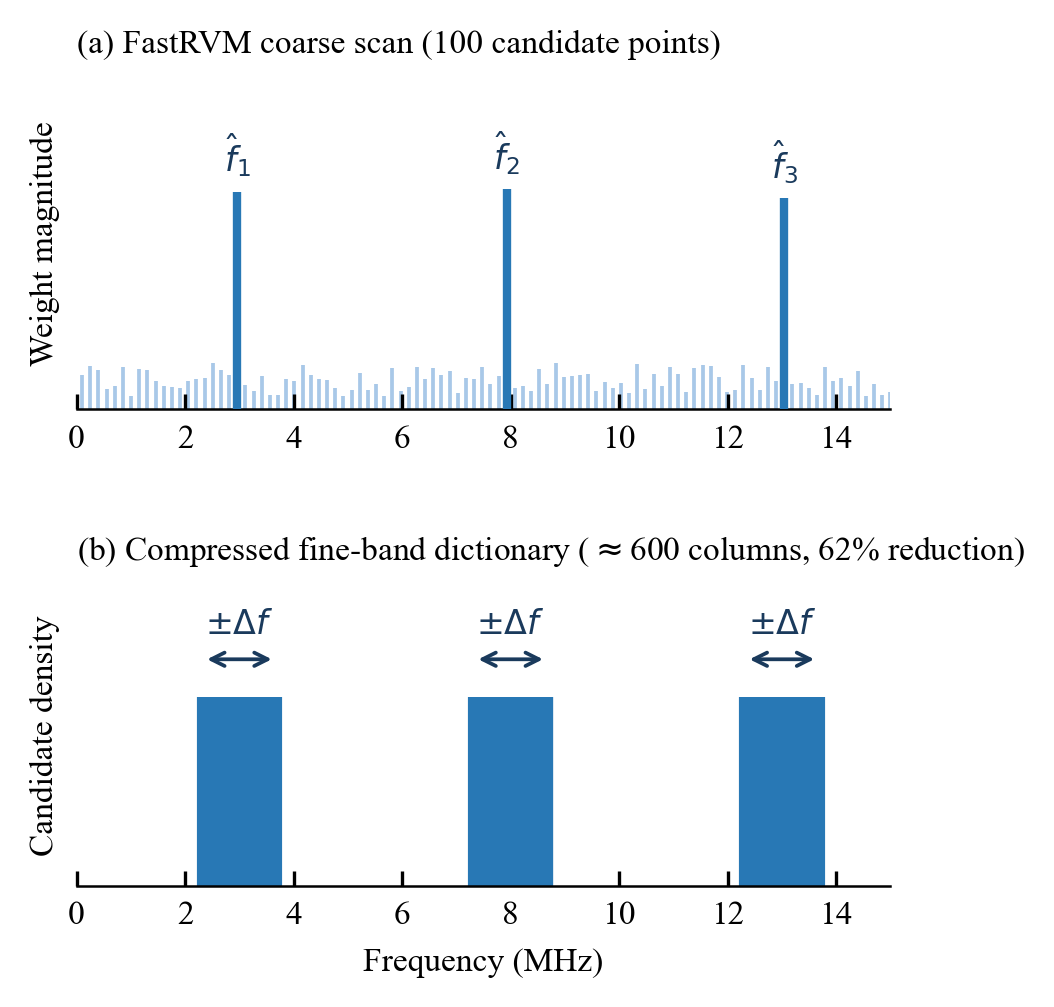
\includegraphics[width=0.88\linewidth]{fig2_fastrvm_compression.png}
    \caption{FastRVM coarse localisation and ARD fine-dictionary construction.}
    \label{fig:fastrvm}
\end{figure}

\subsection{Fine frequency identification based on ARD}

The frequency resolution of FastRVM on the coarse grid is approximately 150~kHz, so the obtained $\hat{f}_1, \hat{f}_2, \hat{f}_3$ are only approximate positions of the true frequencies; a fine dictionary must be constructed in their neighbourhoods to yield accurate frequency and amplitude estimates. A fine window of $\pm200$~kHz is expanded around each of $\hat{f}_1, \hat{f}_2, \hat{f}_3$, covering the FastRVM coarse localisation error (approximately $\pm 75$~kHz) and ensuring that the true PJ frequencies fall within the windows. Within each window, 100 candidate frequencies are uniformly sampled with a spacing of approximately 4~kHz; the three windows are merged to yield 300 fine candidate frequencies. A fine global dictionary $\mathbf{H} \in \mathbb{R}^{N \times M}$ is constructed according to (3)--(5), with $M = 600 + 1 + 32 = 633$ (as illustrated in Fig.~\ref{fig:fastrvm}(b)).

Adjacent candidate frequency columns in the fine dictionary are highly correlated and direct least-squares solution is numerically unstable. Imposing the same ARD prior as in (8) on $\mathbf{H}$, the conjugacy between the Gaussian prior and the Gaussian observation model gives a Gaussian posterior $p(\mathbf{w} \mid \mathbf{y})$ with mean and covariance:

\begin{equation}
\boldsymbol{\mu} = \sigma^{-2}\boldsymbol{\Sigma}\mathbf{H}^T\mathbf{y}, \quad \boldsymbol{\Sigma} = \left(\sigma^{-2}\mathbf{H}^T\mathbf{H} + \boldsymbol{\Lambda}\right)^{-1} \tag{12}
\end{equation}

where $\boldsymbol{\Lambda} = \mathrm{diag}(\alpha_1, \ldots, \alpha_M)$. The posterior mean $\boldsymbol{\mu}$ serves as the coefficient estimate.

The hyperparameters $\{\alpha_i\}$ and noise variance $\sigma^2$ are not manually specified but are jointly estimated from the data by maximising the marginal likelihood $p(\mathbf{y} \mid \{\alpha_i\}, \sigma^2)$, with update rules:

\begin{equation}
\alpha_i^{\mathrm{new}} = \frac{1 - \alpha_i \Sigma_{ii}}{\mu_i^2}, \quad (\sigma^2)^{\mathrm{new}} = \frac{\|\mathbf{y} - \mathbf{H}\boldsymbol{\mu}\|^2}{N - \sum_i(1 - \alpha_i\Sigma_{ii})} \tag{13}
\end{equation}

where $\Sigma_{ii}$ is the $i$-th diagonal element of the posterior covariance matrix. The updates of $\alpha_i$ and $\sigma^2$ alternate until convergence.

After inference convergence, the posterior mean $\boldsymbol{\mu}$ is used directly as the coefficient estimate for each component: the coefficient pair $(\hat{a}_i, \hat{b}_i)$ at an active frequency yields the PJ peak-to-peak value via (6); the DCD and ISI column coefficients give the corresponding component amplitudes; and the RJ RMS is estimated from the residual via (7).


\section{Experimental Validation}

To verify the effectiveness of the proposed method, simulation experiments are designed to evaluate the wide-band PJ estimation accuracy and the multi-component joint decomposition accuracy, comparing LS-FFT~\cite{duan_fast_2019} against the proposed SBL method. The simulated data are TIE sequences generated under PRBS-7 patterns at a 2~Gbps data rate, with 50{,}000 samples collected, channel memory depth $L=5$, and DCD and ISI ground truths set to 1.0~ps and 0.16~ps respectively. Since the FFT peak shift varies with the PJ frequency, the experiments scan the PJ frequency over 100~kHz--15~MHz to compare the decomposition performance of the two methods. Two parameter sets are used: Sample~1 with PJ = 10.0~ps and RJ = 5.0~ps; Sample~2 with PJ = 6.0~ps and RJ = 5.0~ps.

Six frequency points (0.1, 0.5, 1, 5, 10 and 15~MHz) are selected within 100~kHz--15~MHz, and the peak-to-peak PJ estimation errors of the two parameter sets are shown in Fig.~\ref{fig:freq_accuracy}.

\begin{figure}[!ht]
    \centering
    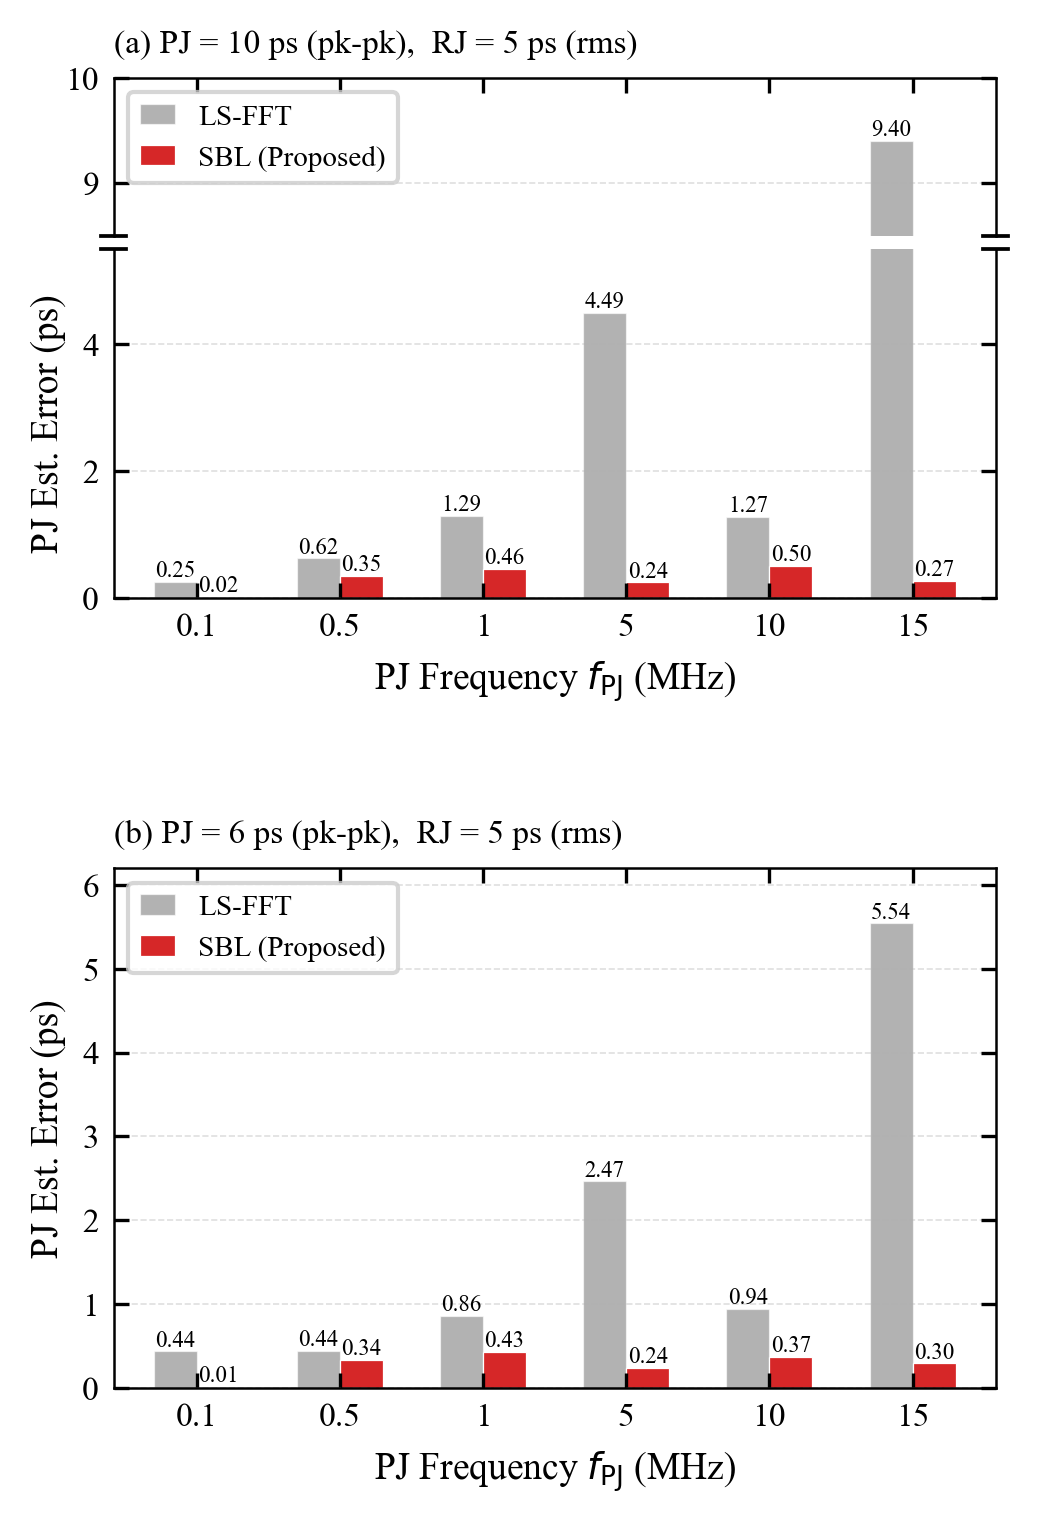
\includegraphics[width=0.9\linewidth]{fig4_freq_accuracy_combined.png}
    \caption{Wide-band PJ estimation errors for the two samples.}
    \label{fig:freq_accuracy}
\end{figure}

As shown in Fig.~\ref{fig:freq_accuracy}, in both samples and at all six frequency points the SBL PJ error remains below 0.5~ps with no clear dependence on frequency, whereas the LS-FFT PJ error grows with frequency and reaches 9.40~ps (Sample~1) and 5.54~ps (Sample~2) at 15~MHz, exceeding the SBL error by one to two orders of magnitude. This is because the LS-FFT PJ error is dominated by the FFT frequency-estimation bias: the higher the frequency, the larger the relative shift between adjacent DFT bins, and the larger the resulting estimation error. SBL identifies the active frequencies directly from the redundant dictionary and does not rely on the uniform-sampling assumption, so its error does not vary with frequency.

Three frequency points (0.1, 1.0 and 10.0~MHz) are then chosen to compare the simultaneous decomposition accuracy of the four components---PJ, DCD, ISI and RJ---and the errors are reported in Table~\ref{tab:decomp_err}.

\begin{table*}[!t]
\caption{Multi-component decomposition errors (ps). Ground truth---Sample~1: PJ = 10.00, DCD = 1.00, ISI = 0.16, RJ = 5.00; Sample~2: PJ = 6.00, DCD = 1.00, ISI = 0.16, RJ = 5.00.}
\label{tab:decomp_err}
\centering
\begin{tabular*}{\textwidth}{@{\extracolsep{\fill}} ll cccc cccc}
\hline
 & & \multicolumn{4}{c}{LS-FFT Error (ps)} & \multicolumn{4}{c}{SBL Error (ps)} \\
\cmidrule(lr){3-6}\cmidrule(lr){7-10}
Sample & $f_{PJ}$ & PJ & DCD & ISI & RJ & PJ & DCD & ISI & RJ \\
\hline
\multirow{3}{*}{1} & 0.1 MHz  & 0.25 & 0.04 & 0.41 & 0.01 & 0.02 & 0.03 & 0.30 & 0.01 \\
                   & 1.0 MHz  & 1.29 & 0.04 & 0.48 & 0.06 & 0.46 & 0.03 & 0.30 & 0.01 \\
                   & 10.0 MHz & 1.28 & 0.04 & 0.44 & 0.55 & 0.50 & 0.03 & 0.30 & 0.02 \\
\hline
\multirow{3}{*}{2} & 0.1 MHz  & 0.44 & 0.04 & 0.42 & 0.01 & 0.01 & 0.03 & 0.30 & 0.01 \\
                   & 1.0 MHz  & 0.86 & 0.04 & 0.44 & 0.01 & 0.43 & 0.03 & 0.30 & 0.01 \\
                   & 10.0 MHz & 0.94 & 0.04 & 0.42 & 0.20 & 0.37 & 0.03 & 0.30 & 0.02 \\
\hline
\end{tabular*}
\end{table*}

As shown in Table~\ref{tab:decomp_err}, in both samples and at all three frequency points the SBL PJ error stays within 0.50~ps, while the DCD and RJ errors are bounded by 0.03~ps and 0.02~ps respectively. The LS-FFT PJ error reaches 1.28~ps (Sample~1) and 0.94~ps (Sample~2) at 10.0~MHz, and at this frequency the RJ error of Sample~1 rises to 0.55~ps, indicating that the LS-FFT frequency shift misaligns the PJ basis functions with the true signal so that the unfit PJ energy spills into the residual and biases the RJ estimate. The SBL RJ estimate stays close to its ground truth at all settings, confirming that accurate frequency identification cuts off this cross-component error propagation. Both methods over-estimate the ISI by approximately 0.30~ps regardless of the PJ frequency, which is caused by finite-sample statistical accumulation of RJ noise when the conditional means of $\mathbf{C}$ are taken over its $2^L = 32$ pattern bins; this bias is intrinsic to the ISI sub-model and unrelated to the frequency identification.

To visualise the decomposition quality of SBL, the result of Sample~2 at $f_{PJ} = 1$~MHz is shown in Fig.~\ref{fig:decomp_vis}.

\begin{figure}[!ht]
    \centering
    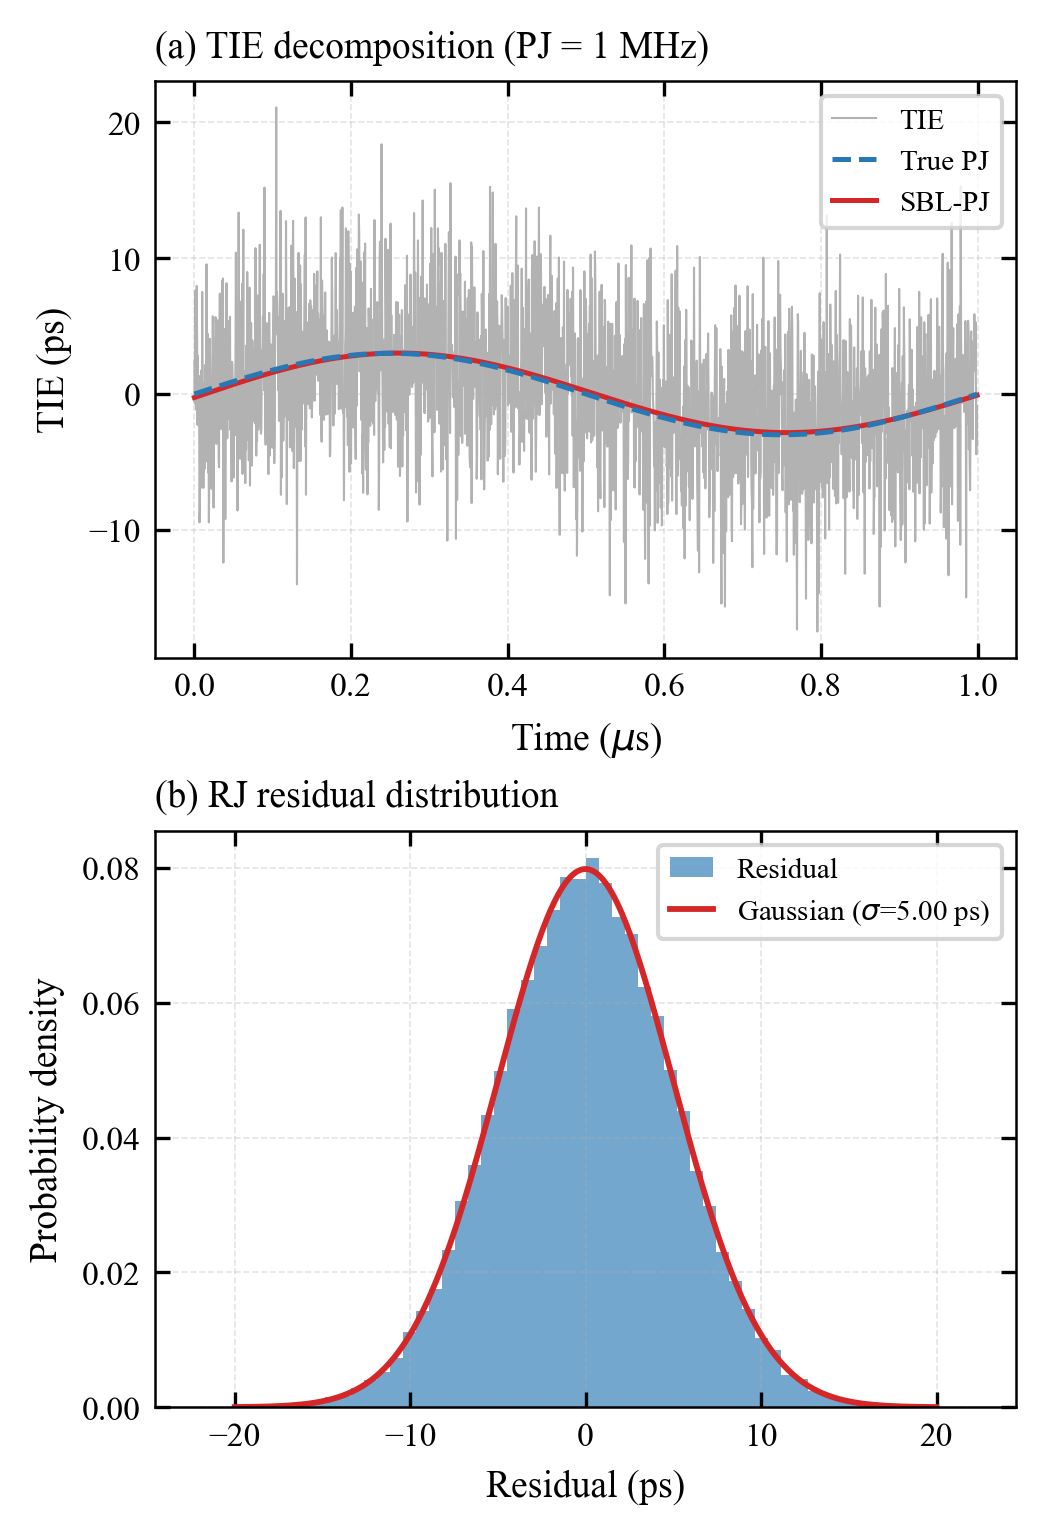
\includegraphics[width=0.9\linewidth]{fig5_decomposition.png}
    \caption{SBL decomposition result at $f_{PJ} = 1$~MHz.}
    \label{fig:decomp_vis}
\end{figure}

In Fig.~\ref{fig:decomp_vis}(a), the SBL-recovered PJ curve almost perfectly overlaps the ground-truth sinusoid in phase, amplitude and period, with no frequency offset or envelope mismatch---confirming that the frequency column identified by ARD from the 600-column fine dictionary corresponds to the 1~MHz ground truth and that the coefficient pair $(\hat{a}, \hat{b})$ accurately recovers the cosine and sine amplitudes. In Fig.~\ref{fig:decomp_vis}(b), the residual histogram agrees closely with a zero-mean Gaussian distribution of $\sigma = 5.00$~ps, with no long tail or non-Gaussian structure, indicating that the deterministic components have been fully absorbed by the dictionary sub-matrices and have not leaked into the residual.




\section{Conclusion}

This paper proposes a jitter multi-component decomposition method based on Sparse Bayesian Learning, which addresses the frequency estimation bias of LS-FFT on PRBS non-uniform TIE sequences. Building on the linear superposition model of LS-FFT, the proposed method replaces the single-frequency column with a redundant frequency dictionary and exploits the ARD mechanism to directly identify the true PJ frequencies from the dictionary, without requiring any prior frequency knowledge. Compared with LS-FFT, the proposed method's frequency estimation is no longer affected by non-uniform TIE sequences, the PJ estimation accuracy remains stable across the wide band, and the propagation of frequency bias into the RJ component is suppressed, improving the reliability of jitter decomposition under PRBS non-uniform sampling. Future work will further validate the engineering applicability of the proposed method on measured oscilloscope data.


% --- 参考文献 ---

\begin{thebibliography}{99}

\bibitem{balestrieri_review_2019} Balestrieri, E., Picariello, F., Rapuano, S., Tudosa, I.: `Review on jitter terminology and definitions', \textit{Measurement}, 2019, \textbf{145}, pp.~264--273

\bibitem{chen_methodology_2023} Chen, J., Ye, P., Zhao, Y., Zhang, Q., Huang, C.: `Methodology for jitter analysis in digital storage oscilloscope'. Proc.\ 2023 IEEE 16th Int.\ Conf.\ Electronic Measurement \& Instruments (ICEMI), Aug.\ 2023, pp.~1--6

\bibitem{tripathi_review_2018} Tripathi, J.N., Sharma, V.K., Shrimali, H.: `A review on power supply induced jitter', \textit{IEEE Trans. Compon. Packag. Manuf. Technol.}, 2019, \textbf{9}, (3), pp.~511--524

\bibitem{deng_jitter_2024} Deng, Y., Shang, Z., Tang, Z., Hou, T., Liu, W., Bin, S., Chen, X.: `Jitter analysis and decomposition based on tail-fit algorithm'. Proc.\ 2024 4th Int.\ Conf.\ Communication Technology and Information Technology (ICCTIT), Guangzhou, China, Dec.\ 2024, pp.~611--615

\bibitem{fang_jitter_2024} Fang, S., Pan, W., Pan, D., Xu, Z., Gao, Z., Zhao, T.: `Jitter analysis based on kernel density estimation and dual-Dirac'. Proc.\ 2024 IEEE Int.\ Conf.\ Signal, Information and Data Processing (ICSIDP), Zhuhai, China, Nov.\ 2024, pp.~1--6

\bibitem{peng_jitter_2025} Peng, J., Qi, Z., Li, Z., Sun, Q., Pan, D., Zhao, T.: `Jitter decomposition based on dual-Dirac model: a two-stage limited-sampling algorithm'. Proc.\ 2025 IEEE 17th Int.\ Conf.\ Electronic Measurement \& Instruments (ICEMI), Beijing, China, Aug.\ 2025, pp.~169--174

\bibitem{dou_jitter_2006} Dou, Q., Abraham, J.A.: `Jitter decomposition by time lag correlation'. Proc.\ 7th Int.\ Symp.\ Quality Electronic Design (ISQED), San Jose, CA, USA, Mar.\ 2006, pp.~525--530

\bibitem{yamaguchi_fft_2007} Yamaguchi, T.J., Ishida, M., Hou, H.X., et al.: `An FFT-based jitter separation method for high-frequency jitter testing with a 10$\times$ reduction in test time'. Proc.\ IEEE Int.\ Test Conf.\ (ITC), Santa Clara, CA, USA, Oct.\ 2007, pp.~1--8

\bibitem{ren_jitter_2021} Ren, N., Fu, Z., Zhou, D., et al.: `Jitter decomposition by convolutional neural networks', \textit{IEEE Trans. Electromagn. Compat.}, 2021, \textbf{63}, (4), pp.~1550--1561

\bibitem{duan_fast_2019} Duan, Y., Chen, D.: `Fast and accurate decomposition of deterministic jitter components in high-speed links', \textit{IEEE Trans. Electromagn. Compat.}, 2019, \textbf{61}, (1), pp.~217--225

\bibitem{tipping_sparse_2001} Tipping, M.E.: `Sparse Bayesian learning and the relevance vector machine', \textit{J. Mach. Learn. Res.}, 2001, \textbf{1}, pp.~211--244

\bibitem{faul_analysis_2001} Faul, A.C., Tipping, M.E.: `Analysis of sparse Bayesian learning', in Dietterich, T.G., Becker, S., Ghahramani, Z. (Eds.): `Advances in Neural Information Processing Systems 14' (MIT Press, Cambridge, MA, 2002), pp.~383--389

\end{thebibliography}

\end{document}
